\documentclass[aspectratio=169, 11pt]{beamer}
\usepackage[utf8]{inputenc}
\usepackage[spanish]{babel}
\usepackage{amsmath,amsfonts,amsthm,amssymb,mathtools,sectsty}
\pagenumbering{gobble}
\usepackage{subcaption}
%\usepackage{graphicx}
%\usepackage[pdftex,dvipsnames]{xcolor}
\usepackage{cancel}
\usepackage{graphicx}
\usepackage{marginnote}
\usepackage{mathabx}
\usepackage{float}
\setlength{\marginparwidth}{2cm}

% Tikz y las librerías para automátas
\usepackage{tikz-cd}
\usepackage{tikz}
\usetikzlibrary{arrows,automata}
\usetikzlibrary{babel} %para evitar que se jodan los automatas de tikz
\usetikzlibrary{graphs} 
\usetikzlibrary{calc}
\usetikzlibrary{positioning}
%\usetikzlibrary{shapes.geometric}  % for [ellipse], [diamond], etc

%\usepackage[backend=biber,...]{biblatex} 

%Referencias; me gustaría que backref funcione pero no es importante tampoco.
\usepackage[pagebackref]{hyperref}
% Para modificar el estilo de las referencias
\hypersetup{
	colorlinks,
	linkcolor={astral},
	citecolor={red!70!black},
	urlcolor={red!80!black}
}
\definecolor{astral}{RGB}{46,116,181}
\colorlet{chulo}{blue!70!purple}
\colorlet{rojo}{purple!45!black}
\definecolor{carrotorange}{rgb}{0.93, 0.57, 0.13}
\definecolor{brightcerulean}{rgb}{0.11, 0.67, 0.84}
\definecolor{brightube}{rgb}{0.82, 0.62, 0.91}
\definecolor{cadmiumred}{rgb}{0.89, 0.0, 0.13}
\definecolor{applegreen}{rgb}{0.55, 0.71, 0.0}
\definecolor{aurometalsaurus}{rgb}{0.43, 0.5, 0.5}

%%%%%%%%%%%%%%%%%%%%% ENUMERAR CON COSAS QUE NO SEAN SOLO NÚMEROS %%%%%%%%%%
\usepackage[shortlabels]{enumitem}
\setlist[enumerate]{font=\bfseries}
\usepackage{adjustbox}


%%%%%%%%%%%%%%%%%%%%%%% TÍTULOS DE SECCIONES MÁS FANCIES %%%%%%%%%%%%%%
\usepackage{titlesec}
\setcounter{secnumdepth}{3} % Hasta que profundidad quiero numerar, 4 sería los párrafos.
\titleformat{\section}[block]{\color{astral!50!black}\Large\bfseries\filcenter}{\S\thesection.}{1em}{}
\titleformat{\subsection}[hang]{\color{astral!50!black}\large\bfseries\filcenter}{\S\thesubsection.}{1em}{}

%%%%%%%%%%%%%%%%%%%%%% COLORES PÁRRAFOS Y CAPÍTULOS %%%%%%%%%%%%%%%%%%%%%%%%
%\paragraphfont{\color{astral!70!black}}
\chapterfont{\color{astral!40!black}}
%\subsectionfont{\color{astral!60!black} }
%\sectionfont{\color{astral!50!black} }

\usepackage{mathpazo}
\usepackage{amssymb}
%\usepackage{thmtools}

%Esto sirve para armar grafos de Cayley de una manera más copada.
\usetikzlibrary{lindenmayersystems,arrows.meta}
\pgfdeclarelindenmayersystem{cayley}{
	\rule{G->G-G+++G--G}
	\symbol{R}{
		\pgflsystemstep=0.5\pgflsystemstep
	}

}

\usepackage[framemethod=tikz]{mdframed}

%%%%%%%%%%%%%  TEOREMAS  %%%%%%%%%%%%%%%%%
\theoremstyle{plain} %% el estilo clásico
\newtheorem{teo}{\color{rojo}{ { Teorema}}}[section]
\newtheorem{prop}[teo]{\color{rojo} {Proposición}}
\newtheorem{lema}[teo]{\color{rojo} {Lema}}
\newtheorem{coro}[teo]{\color{rojo} {Corolario}}
\newtheorem*{aff}{ {Afirmación}}
% Si pongo [theorem] siguen la numeración de los teoremas. 
% e.j. Teo 1, Lema 2, Teo 3, Teo 4 ...
\theoremstyle{definition}
\newtheorem{deff}[teo]{{ Definición}}{\smallskip}
\newtheorem{ej}[teo]{{Ejemplo}}{\smallskip}

% Remarks
\theoremstyle{remark}
\newtheorem{obs}[teo]{ {Observación}}{\smallskip}

%%%%%%%%%% FRAMES PARA TEOREMAS A LO HATCHER %%%%%%%%%%%%%%%%%%%%%%%%%

\surroundwithmdframed[outerlinewidth=0.4pt,
innerlinewidth=0.4pt,
align=center,
middlelinewidth=1pt,
middlelinecolor=white,
innertopmargin=-4pt,
innerbottommargin=0pt,
innerrightmargin=4pt,
innerleftmargin=4pt,
bottomline=false,topline=false,rightline=false]{teo}
\surroundwithmdframed[outerlinewidth=0.4pt,
innerlinewidth=0.4pt,
align=center,
middlelinewidth=1pt,
middlelinecolor=white,
innertopmargin=-4pt,
innerbottommargin=0pt,
innerrightmargin=4pt,
innerleftmargin=4pt,
bottomline=false,topline=false,rightline=false]{lema}

\surroundwithmdframed[outerlinewidth=0.4pt,
innerlinewidth=0.4pt,
align=center,
middlelinewidth=1pt,
middlelinecolor=white,
innertopmargin=-4pt,
innerbottommargin=0pt,
innerrightmargin=4pt,
innerleftmargin=4pt,
bottomline=false,topline=false,rightline=false]{prop}


\surroundwithmdframed[outerlinewidth=0.4pt,
innerlinewidth=0.4pt,
align=center,
middlelinewidth=1pt,
middlelinecolor=white,
innertopmargin=-4pt,
innerbottommargin=0pt,
innerrightmargin=4pt,
innerleftmargin=4pt,
bottomline=false,topline=false,rightline=false]{coro}

%==================================================================%

% DEMOS EN NEGRITA.
\renewenvironment{proof}{{\textbf{Demostración.}}}{ \hfill $\blacksquare$ \medskip} 

%% ========== Para escribir pseudo ==========
%\usepackage{algorithm}
%\usepackage[noend]{algpseudocode}  % "noend" es para no mostrar los endfor, endif
%%\algrenewcommand\alglinenumber[1]{\tiny #1:}  % Para que los numeros de linea del pseudo sean pequeños
%\renewcommand{\thealgorithm}{}  % Que no aparezca el numero luego de "Algorithm"
%\floatname{algorithm}{ }    % Entre {  } que quiero que aparezca en vez de "Algorithm"
%
%% traducciones
%\algrenewcommand\algorithmicwhile{\textbf{mientras}}
%\algrenewcommand\algorithmicdo{\textbf{hacer}}
%\algrenewcommand\algorithmicreturn{\textbf{devolver}}
%\algrenewcommand\algorithmicif{\textbf{si}}
%\algrenewcommand\algorithmicthen{\textbf{entonces}}
%\algrenewcommand\algorithmicfor{\textbf{para}}
%
%%% indentar dentro de los algoritmos
%\algdef{SE}[SUBALG]{Indent}{EndIndent}{}{\algorithmicend\ }%
%\algtext*{Indent}
%\algtext*{EndIndent}

% =========================================================
\usepackage[colorinlistoftodos,prependcaption,textsize=tiny]{todonotes}



%Comandos útiles.
\newcommand\RP{\mathbb{RP}}
\newcommand{\norm}[1]{\left\lVert#1\right\rVert}
\newcommand{\RR}{\mathbb{R}}
\newcommand{\CC}{\mathbb{C}}
\newcommand{\NN}{\mathbb{N}}
\newcommand{\ZZ}{\mathbb{Z}}
\newcommand{\Om}{\Omega}
\newcommand{\A}{\mathcal A}
\newcommand\ol{\overline}
\newcommand{\blue}{\textcolor{chulo}}
\newcommand{\red}{\textcolor{rojo}}
\newcommand{\Gg}{\mathfrak g}
\newcommand{\SL}{SL_2(\mathbb Z)}
\newcommand{\stab}{\text{Stab}}
\newcommand{\ic}{independiente de contexto }
\newcommand{\APND}{automáta de pila no determinístico }
\newcommand{\APD}{automáta de pila determinístico }
\newcommand{\gramatica}{{\cal G} = (V, \Sigma, P, S)}
\newcommand{\deriva}{\overset{*}{\to_{\cal G}}}
\newcommand{\tto}{\overset{*}{\to}}
\newcommand{\lengderivado}{L({\cal G})}
\newcommand{\fg}{grupo finitamente generado }
%\newcommand{\ol}{\overline{}}
\newcommand{\aut}{\text{Aut}}
\newcommand{\Sy}{\text{Sym}} 

\newcommand{\cay}[2]{\text{Cay}(#1,#2)}

\newcommand{\partes}[1]{{\cal{P}}(#1)} 

\newcommand*{\deri}{{\cal D}}
\newcommand*{\lexorder}{\le_{\textrm{lex}}}


\newcommand{\fp}{grupo finitamente presentado }
\newcommand{\vl}{virtualmente libre }
\newcommand{\vls}{virtualmente libres}
\newcommand{\WP}{\text{WP}(G, \Sigma)}

\newcommand{\cG}{ {\cal G} }
\newcommand{\cGg}{{\cal G} = (V, \Sigma, P, S)}
\newcommand{\cH}{ {\cal H} }
\newcommand{\Xm}{\widetilde X}
%\newcommand{\ol}{\overline{}}

%%% Capítulo 5. Cortes.
\newcommand{\olc}[1]{#1^{c}}
\newcommand{\ca}{{\cal C}(\alpha)}
\newcommand{\cmin}{{\cal C}_{\text{min}}}
\newcommand{\cam}{{\cal C}_{\text{min}}(\alpha)}
\newcommand{\copta}{{\cal C}_{\text{opt}}(\alpha)}
\newcommand{\copt}{{\cal C}_{\text{opt}}}
\newcommand*{\rows}{6}

\newcommand{\TODO}[1]{\textcolor{red}{TODO: #1}}

\newenvironment{leoenv}{\color{brightcerulean}}{\ignorespacesafterend}
%%%%%%%%%%%%%%  SETUP DE LA PÁGINA %%%%%%%%%%%%%%%%%
%\usepackage{fancyhdr} 
\pagestyle{headings} 
\pagenumbering{arabic} 
%\foot[C]{\textbf{\thepage}} % except the center
%\setlength{\headheight}{42pt}% ...at least 51.60004pt
%\renewcommand{\headrulewidth}{0.8pt}
%\head[L]{\thepage} 
%\head[R]{\textsl{\leftmark}} 
%\fancyfoot[C]{\thepage}

\usepackage{float}


\usepackage{subfiles} % mejor ponerlos al final


\title{El problema de la palabra de los grupos virtualmente libres.}
\subtitle{\textbf{Leopoldo Lerena} \\
		Defensa de tesis de licenciatura.}
\date{??.}
\author{Director: Iván Sadofschi Costa}
\institute{Universidad de Buenos Aires}
% \titlegraphic{\hfill\includegraphics[height=1.5cm]{logo.pdf}}

\begin{document}
	\maketitle

	
	
	
	\begin{frame}[fragile]{Problema de la palabra.}
		Sea $G$ un grupo \fg por un conjunto finito $A$; 
		tal que $G$ es isomorfo a $\langle A \mid R \rangle$ para un conjunto de relaciones $R \subseteq (A \cup A^{-1})^*$.
		
		El \emph{problema de la palabra} consiste en el siguiente problema:
	
		\begin{itemize}
					\item 
						\textbf{Entrada}: Una palabra $w \in (A \cup A^{-1})^*$.
					
					\item 
						\textbf{Pregunta}: Decidir si vale $w=1$ en $G$.
		\end{itemize}

		El problema de la palabra no es un problema \alert{decidible}.
		\begin{itemize}
			\item 
				Existen grupos tales que resulta imposible construir un algoritmo que decida si una palabra representa la identidad o no.
		\end{itemize}
		

	\end{frame}

	\begin{frame}[fragile]{Grafo de Cayley.}
		Dado un grupo $G$ finitamente generado por $A$ podemos considerar un grafo $\Gamma =\cay{G}{A}$ que es el grafo de Cayley.

		Está definido de manera que 
		\[
			V(\Gamma) = G,   \ \ \ E(\Gamma) = \{ \{ g,ga \}  \mid g \in G, a \in A \cup A^{-1}  \}. 	
		\]

		\TODO{Agregar el dibujo del grafo de Cayley de un grupo.}
	\end{frame}
	
	\begin{frame}[fragile]{Grupos libres.}
		Dado un conjunto $A$ notamos $F_{A}$ al \emph{grupo libre} generado por los elementos de $A$. 

		% \onslide<2->
		El grupo $F_{A}$ viene con una función $\iota: A \to F_{A}$ que denominamos la inclusión de los generadores en el grupo libre y queda caracterizado por la siguiente propiedad universal: 
		Para todo grupo $H$ y toda función $f:A \to H$ existe un único morfismo de grupos $\ol f: F_{A} \to H$ tal que $\ol f \circ \iota = f$.
		\begin{center}
			\begin{tikzcd}
				F_{A}  \arrow[rr, "\ol f", dashed]          &  & H \\
				&  &   \\
				A \arrow[uu, "\iota"] \arrow[rruu, "f", swap] &  &  
			\end{tikzcd}
		\end{center}

		% \onslide<3->
		Decimos que $A$ genera libremente a $F_{A}$ y que $A$ es una base de $F_{A}$.

		% \onslide<4->
		Podemos identificar los elementos de $F_{A}$ con las palabras reducidas en $A \cup A^{-1}$.
	\end{frame}

	\begin{frame}[fragile]{Grupos virtualmente libres.}
		Un grupo $G$ es \emph{virtualmente libre} si es finitamente generado y si
		tiene un subgrupo libre $F$ tal que $[G:F] < \infty$.

		\begin{alertblock}{Ejemplos.}
			\begin{itemize}
				\item Los grupos finitos.
				\item Los grupos libres.
				\item El producto semidirecto de un grupo libre con un grupo finito.
				\item El producto libre de dos grupos finitos.
			\end{itemize}
		\end{alertblock}
	\end{frame}

	\begin{frame}[fragile]{Teoría de lenguajes.}
		Dado un conjunto finito $A$ notaremos por $A^*$ al monoide libre sobre $A$.
		
		\begin{deff}
			Un lenguaje $L$ sobre un alfabeto $A$ es un subconjunto de $A^*$.
		\end{deff}	
		
		\begin{alertblock}{Ejemplos.}
			\begin{itemize}
				\item 
					Dado $\Sigma = \{a,b\}$ consideramos el lenguaje de los palíndromos
					\[
						L = \{ w \in \Sigma^{*} \mid w = w^{R}  \}.
					\]
				\item 
					Dado un grupo $G$ finitamente generado por $A$ consideramos el lenguaje
					\[
						\WP{G}{A} = \{ w \in (A \cup A^{-1})^{*} \mid w = 1 \ \text{en $G$} \}.	
					\]
			\end{itemize}
		\end{alertblock}
	\end{frame}
	
	\begin{frame}[fragile]{Ejemplo de gramática.}
		Consideramos las siguientes reglas.
		\begin{align*}
			S  & \to aAS \mid b \\
			A  & \to baAb \\
			aA & \to bbb
		\end{align*}
		Entonces aplicamos estas reglas para generar la siguiente palabra.
		\[
			S \to aAS \to abaAbS \to abaAbb \to abbbbbb	
		\]
	\end{frame}

	\begin{frame}[fragile]{Gramáticas (pt.1).}
		\begin{deff}
			Una \emph{gramática} es una tupla ${\cal G} = (V, \Sigma, P, S)$ donde:
				\begin{itemize}
					\item $V$ es un conjunto finito denominado las \emph{variables};
					\item $\Sigma$ es un conjunto finito disjunto de $V$ que denominamos \emph{símbolos terminales};
					\item $P \subseteq (V \cup \Sigma)^*V(V \cup \Sigma)^* \times (V \cup \Sigma)^*$ es un conjunto finito de \emph{producciones}.
					
					Las producciones $(\gamma, \nu) \in P$, las denotamos por medio de la siguiente notación $\gamma \to \nu$.
					\item $S \in V$ es el \emph{símbolo inicial};
				\end{itemize}
		\end{deff}
	\end{frame}
	
	\begin{frame}[fragile]{Gramáticas (pt.2).}
		Una sucesión de producciones $\gamma_{1} \to \gamma_{2} \to \dots \gamma_{n}$ la denotamos $\gamma_{1} \to^{*} \gamma_{n}$ y diremos que es un \emph{derivación}.

		\begin{deff}
			Dada una gramática $\cGg$  definimos el \emph{lenguaje generado por la gramática} como
			\[
			L({\cal G}) = \{ w \in \Sigma^* \ | \ S \deriva w   \}.
			\]
		\end{deff}		
	\end{frame}

	\begin{frame}{Gramáticas regulares.}
		\begin{deff}
			Decimos que una gramática $\gramatica$ es \emph{regular} si las producciones son del estilo
	\begin{enumerate}
		\item $A \to \epsilon$
		\item $A \to a$
		\item $A \to a B$
	\end{enumerate}
	donde $A, B \in V$, $a \in \Sigma$ y $\epsilon$ es la palabra vacía. 

	Si $L=\lengderivado$ para alguna gramática regular $\cal G$ entonces diremos que $L$ es un \emph{lenguaje regular}.
		\end{deff}
	\end{frame}

	\begin{frame}{Gramáticas independiente de contexto.}
		\begin{deff}
			Una gramática $\gramatica $ es \emph{independiente de contexto} si las producciones tienen la siguiente forma:
			\begin{equation*}
				A \to w
			\end{equation*}
			donde $A \in V, w \in (\Sigma \cup V)^*$.  
			
			Si $L=\lengderivado$ para alguna gramática independiente de contexto $\cal G$ entonces diremos que $L$ es un \emph{lenguaje independiente de contexto}.

			\TODO{Comentar porqué se llama independiente de contexto.}
		\end{deff}
		
	\end{frame}

	\begin{frame}{Jerarquía de Chomsky.}

			\centering
			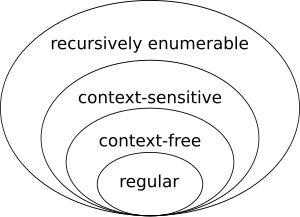
\includegraphics[scale = 0.65]{Chomsky-hierarchy.png}
		
	\end{frame}

	\begin{frame}[fragile]{Clasificación del problema de la palabra.}
		
		\begin{teo}[Animisov--1971]
			Un grupo $G$ es finito si y solo sí $\WP{G}{A}$ es regular.
		\end{teo}
		
		\[
			\begin{tikzpicture}[scale=0.7,->,>=stealth',shorten >=1pt,auto,node distance=3.5cm,
				scale = 1,transform shape]
				\node[state,initial,accepting] (1) [] {$1$};
				\node[state] (a) [above right of=1] {$a$};
				\node[state] (b) [below right of=1] {$b$};
				\node[state] (ab) [below right of=a] {$ab$};

					\path (1) edge    [bend left]          node {$a$ \ } (a);
					\path (a) edge    [bend left,swap]          node {$a^{-1}$ \ } (1);
					\path (1) edge    [bend left]          node {$b$ \ } (b);
					\path (b) edge    [bend left, swap]          node {$b^{-1}$ \ } (1);
					\path (a) edge    [bend left]          node {$b$ \ } (ab);
					\path (ab) edge   [bend left, swap]          node {$b^{-1}$} (a);
					\path (b) edge    [bend left]          node {$a$ \ } (ab);
					\path (ab) edge   [bend left, swap]          node {$a^{-1}$ \ } (b);
			\end{tikzpicture}	
		\]

		\begin{alertblock}{Pregunta natural.}
			¿Es posible caracterizar a los grupos cuyo lenguaje del problema de la palabra es independiente de contexto?
		\end{alertblock}
	\end{frame}
	
	\begin{frame}[fragile]{Teorema de Muller-Schupp.}
		
		\[	
			\begin{tikzpicture}{scale = 0.75}
				\path 
				(0,0) node(a) [rectangle,draw] {$G$ es isomorfo a $\pi_{1}(\cG,P)$ para $\cG$ un grafo de grupos finito con grupos finitos.}
				(5,-3) node(b) [rectangle,draw] {$\cay{G}{A}$ tiene treewidth finito}
				(0,-6) node(c) [rectangle,draw] {$\WP{G}{A}$ es un lenguaje independiente de contexto}
				(-5,-3) node (d) [rectangle,draw] {$G$ es virtualmente libre};
				\draw   
				(d) edge[<-,line width=1.0pt,"Teorema \ref{teo_karrass_solitar}"] (a) 
				(c) edge[<-,line width=1.0pt,"Teorema \ref{teo_Muller_Schupp}"] (d)
				(b) edge[<-,line width=1.0pt,"Teorema \ref{teo_ic_implica_tw}"] (c)
				(a)  edge[<-,line width=1.0pt,"Teorema \ref{coro_tw_finito_implica_pi1}"] (b);
			\end{tikzpicture}
		\]
	\end{frame}

	\begin{frame}[fragile]{Forma normal de Chomsky.}
		\begin{deff}
			Una gramática $\gramatica$ independiente de contexto está en \emph{forma normal de Chomsky} si las producciones son de este tipo:
			\begin{enumerate}
				\item $A \to BC$ donde $A\in V$ y $B,C \in V \setminus \{ S \}$.
				\item $A \to a$ donde $A \in V, a \in \Sigma$.
				\item $S \to \epsilon$ 
			\end{enumerate}
		\end{deff}
		\begin{alertblock}{Ventaja.}
			Si queremos saber si una palabra $w \in \Sigma^{*}$ con longitud $|w| = n$ es tal que $w \in L(\cG)$ entonces nos basta con mirar todas las derivaciones de longitud al menos $2n-1$.
		\end{alertblock}
	\end{frame}

	\begin{frame}[fragile]{Un lema para forma normal de Chomsky pt 1.}
		
		\begin{columns}
			
			\begin{column}{0.5\textwidth}
				Sea la gramática $\gramatica$ definida por:
				
					 $V = \{ S,A,B,C,D \}$;

					 $\Sigma = \{ a,b,c \}$;
					 
						
						$P = \begin{cases}
								S \to AB \mid CD \mid a \mid b \mid c \\
								A \to CD \mid a \mid b \mid c	\\
								B \to BB \mid a \mid b \mid c	\\
								C \to AB \mid a \mid b \mid c	\\
								D \to DD \mid a \mid b \mid c
						\end{cases}$
						
				
			\end{column}

			\begin{column}{0.5 \textwidth}
				Podemos derivar la palabra $w = caabccab$ del siguiente modo:
				\begin{align*}
					&S \to AB \to CDB \to CDBB \to CDBb \to CDab \to \\
					&ABDab  \to  AbDab   \to AbDDab  \to CDbDDab   \to\\
					&CDbccab  \to CDDbccab \to Caabccab \to caabccab \\
				\end{align*}
			\end{column}
		\end{columns}
	\end{frame}

	
	\begin{frame}{Ejemplo forma normal de Chomsky pt.2}
		Consideremos la subpalabra $u  = aabcc$ de $w = caabccab$.
		Consideremos el \textit{árbol de derivación}.
		\TODO{Agregar dibujito y decir que el nodo tal es el más chico que deriva la subpalabra $u$}. 
		
	\end{frame}

	\begin{frame}[fragile]{Un lema para forma normal de Chomsky pt 2.}
		En general vale el siguiente enunciado.

		\begin{lema}
			Sea $\gramatica$ una gramática independiente de contexto en forma normal de Chomsky.
			Sea $w \in L(\cG)$ tal que $w = tuv$ con $t,u,v \in \Sigma^{*}$. 
			Si fijamos una derivación $S \to^{*} w$ entonces existe un único vértice en el árbol de derivación con la propiedad de ser el más bajo entre aquellos de los que deriva una subpalabra que da lugar a $u$.
		\end{lema}

		\TODO{Agregar oralmente detalles sobre "da lugar a $u$".}
	\end{frame}
	
	\begin{frame}[fragile]{Teorema de Muller--Schupp.}
		\[	
			\begin{tikzpicture}{scale = 0.75}
				\path 
				(0,0) node(a) [rectangle,draw] {$G$ es isomorfo a $\pi_{1}(\cG,P)$ para $\cG$ un grafo de grupos finito con grupos finitos.}
				(5,-3) node(b) [rectangle,draw] {$\cay{G}{A}$ tiene treewidth finito}
				(0,-6) node(c) [rectangle,draw] {$\WP{G}{A}$ es un lenguaje independiente de contexto}
				(-5,-3) node (d) [rectangle,draw] {$G$ es virtualmente libre};
				\draw   
				(d) edge[<-,line width=1.0pt,"Teorema \ref{teo_karrass_solitar}"] (a) 
				(c) edge[<-,line width=1.0pt,"Teorema \ref{teo_Muller_Schupp}"] (d)
				(b) edge[<-,line width=1.0pt,"Teorema \ref{teo_ic_implica_tw}"] (c)
				(a)  edge[<-,line width=1.0pt,"Teorema \ref{coro_tw_finito_implica_pi1}"] (b);
			\end{tikzpicture}
		\]
	\end{frame}

	\begin{frame}{Descomposición en un árbol y treewidth de un grafo.}
	Sea $\Gamma$ un grafo no dirigido.
	Una \emph{descomposición en un árbol} de $\Gamma$ es un par $(T,f)$ donde
	$T$ es un árbol y $f$ una función 
	\[
	f: V(T) \to \partes{V(\Gamma)}
	\]
	Que cumple las siguientes condiciones:
	\begin{enumerate}
		\item Para todo vértice $v \in V(\Gamma)$ debe existir $t \in V(T)$ tal que $v \in f(t)$. 
		\item Para toda arista $\{v,w\} \in E(\Gamma)$ 
		debe existir $t \in V(T)$ tal que $v,w \in f(t)$.
		\item Si $v \in V(\Gamma)$ es tal que $v \in f(t) \cap f(s)$ luego $v \in f(r)$ para todo $r \in V(T)$ en la geodésica que va desde $s$ a $t$.  
	\end{enumerate}
	\end{frame}
	
	\begin{frame}[fragile]{Descomponiendo el grafo de Cayley en un árbol.}
		Dado $\Gamma = \cay{G}{A}$ donde $G$ es finitamente generado por $A$.

		Sea $C \subseteq V(\Gamma)$ definimos:
		\begin{itemize}
			\item  
				La \textit{vecindad de $C$} es el siguiente conjunto:

				$N(C) = C \cup \{ v \in V(\Gamma) \mid \exists w \in C, \ \{v,w \} \in E(\Gamma) \}.$

			\item 
				El \textit{borde de $C$} es el siguiente conjunto: 

				$\beta C =  N(C) \cap N(C^{c})$.
		\end{itemize} 
	\end{frame}

	\begin{frame}[fragile]{Descomponiendo el grafo de Cayley en un árbol pt.2}
		Para cada $n \in \NN_{0}$ consideramos:
		\[
			V_{n} = V(\Gamma \setminus B_{n}(1))	
		\]

		Consideramos el siguiente árbol $T$ con raíz $1$:
		\begin{align*}
			V(T)  & = \{ \beta C \mid C \in V_{n} \ \text{componente conexa} \}  \cup \{ 1 \} \\
			E(T)  =  & \{ \{ \beta C, \beta D \}  \mid C \subseteq D \\ 
			& \text{$C$ es componente conexa de $V_{n+1}$ y $D$ componente conexa de $V_{n}$} \} \\
			& \cup \{ \{1, \beta C\} \mid C \ \text{es componente conexa de $V_{0}$} \}
		\end{align*}
		Definimos $f: V(T) \to \partes{V(\Gamma)}$ por medio de $f(\beta C) = \beta C$.
		\begin{lema}
			El par $(T,f)$ es una descomposición en un árbol para el grafo $\Gamma$.
		\end{lema}
	\end{frame}

	\begin{frame}{Ejemplo de la descomposición en un árbol de un grafo de Cayley (pt. 1).}
	Sea $G = \ZZ / 2\ZZ \ast \ZZ / 3\ZZ $ presentado por 
	$G \simeq \langle a,b \mid a^2, b^3 \rangle$.

	El grafo $\cay{G}{\{ a,b,b^{-1} \}}$ lo representamos de la siguiente manera:
	
	% 	\[
	% 		\begin{tikzpicture}
	% 		[scale=0.60,V/.style = {circle, draw,align= center, minimum size=0.5cm,
	% 				minimum size=2em,inner sep=2,
	% 				 fill=astral!15,font=\scriptsize	},fill fraction/.style={path picture={
	% 						\fill[#1] 
	% 						(path picture bounding box.south) rectangle
	% 						(path picture bounding box.north west);
	% 				}},
	% 		fill fraction/.default=astral!90
	% 		]
	
	% 		\begin{scope}[nodes=V,xshift=4.5cm, yshift=-4cm]
	% 				 \node (1) at (0,0) {$1$};
	% 				\node (a) at (2,0)  {$a$};
	% 				 \node (b) at (-2,2)     {$b$};
	% 				\node (bb) at (-2,-2)    {$b^2$};
	% 				\node (ab) at (4,2)      {$ab$};
	% 				 \node (abb) at (4,-2)     {$ab^2$};
	% 				\node (ba) at (-4,2)     {$ba$};
	% 				\node (bba) at (-4,-2)     {$b^2a$};
	% 				\node (aba) at (6,2)    {$aba$};
	% 				\node (abba) at (6,-2)    {$ab^2a$};
	% 				\node (bab) at (-6,3)    {$bab$};
	% 				\node (babb) at (-6,1)     {$bab^2$};
	% 				\node (bbab) at (-6,-3)     {$b^2ab$};
	% 				\node (bbabb) at (-6,-1)    {$b^2ab^2$};
	% 				\node (abab) at (8,3)    {$abab$};
	% 				\node (ababb) at (8,1)    {$abab^2$};
					
	% 				\node (abbab) at (8,-1)     {$ab^2ab$};
	% 				\node (abbabb) at (8,-3)  {$ab^2ab^2$};
					
	% 			\end{scope}
			
	% 		\draw   (1)  edge[-] (a);
	% 		\draw   (1)  edge[-] (b);
	% 		\draw   (1)  edge[-] (bb);
	% 		\draw   (b)  edge[-] (bb);
	% 		\draw   (b)  edge[-] (ba);
	% 		\draw   (bb)  edge[-] (bba);
	% 		\draw   (a)  edge[-] (ab);
	% 		\draw   (abb)  edge[-] (a);
	% 		\draw   (ab)  edge[-] (abb);
	% 		\draw   (ab)  edge[-] (aba);
	% 		\draw   (aba)  edge[-] (abab);
	% 		\draw   (ababb)  edge[-] (aba);
	% 		\draw   (ababb)  edge[-] (abab);
	% 		\draw   (abb)  edge[-] (abba);
	% 		\draw   (abba)  edge[-] (abbab);
	% 		\draw   (abba)  edge[-] (abbabb);
	% 		\draw   (bba)  edge[-] (bbabb);
	% 		\draw   (bba)  edge[-] (bbab);
	% 		\draw   (ba)  edge[-] (bab);
	% 		\draw   (babb)  edge[-] (bab);
	% 		\draw   (abbab)  edge[-] (abbabb);
	% 		\draw   (ba)  edge[-] (babb);
	% 		\draw   (bbabb)  edge[-] (bbab);
	% 		\draw   (abbab)  edge[-] (abbabb);
	% \end{tikzpicture}
	% \]
	\TODO{Latex no le gusta este dibujo en tikz por algún motivo pero igual compila.}
	\end{frame}
	
	\begin{frame}[fragile]{Ejemplo de la descomposición en un árbol de un grafo de Cayley (pt. 2).}
		El árbol $T$ de la descomposición lo representamos de la siguiente manera:

	\[
			\begin{tikzpicture}[scale=0.8, V/.style = {circle, draw,align= center, minimum size=0.5cm,
			minimum size=3em,inner sep=2,
			fill=applegreen!15,font=\scriptsize	},fill fraction/.style={path picture={
				\fill[#1] 
				(path picture bounding box.south) rectangle
				(path picture bounding box.north west);
		}},
		fill fraction/.default=gray!50
		]
		\node[align=center] at (2, -6) {};
		\begin{scope}[nodes=V,xshift=4.5cm, yshift=-4cm]
			\node (1) at (0,0)  {$\{ b,b^2,1 \}$};
			\node (2) at (2,0)  {$1$};
			\node (3) at (4,0)  {$\{ 1,a \}$};
			\node (4) at (-2,3)     {$\{ b,ba \}$};
			\node (5) at (-2,-3)   {$\{b^2,b^2a\}$};
			\node (6) at (6,0)  {$\{ a,ab,ab^2 \}$};
			
			\node (9) at (8,3)  {$\{ab,aba\}$};
			\node (10) at (8,-3)  {$\{ ab^2, ab^2a \}$};
			
		\end{scope}
		
		
		\draw (1) edge[-] (2);
		\draw (2) edge[-] (3);
		\draw (1) edge[-] (5);
		\draw (1) edge[-] (4);
		\draw (3) edge[-] (6);
		\draw (6) edge[-] (9);
		\draw (6) edge[-] (10);
	\end{tikzpicture}
	\]
	\end{frame}

	
	\begin{frame}[fragile]{Independiente de contexto implica treewidth finito (lemas previos).}
		\begin{lema}[1]
			Sea $G$ un grupo \ic con gramática $\gramatica$ de manera que $L(\cG) = WP(G,\Sigma)$.
			Sea $A \in V$ una variable de esta gramática y consideremos el lenguaje
			\[
			L_A = \{ w \in \Sigma^*  \ | \ A \deriva w  \}.
			\]
			Sea $\pi:\Sigma^* \to G$ la proyección del monoide libre al grupo.
			Entonces vale el siguiente resultado:
			dadas palabras $v,v' \in L_{A}$ luego $\pi(v) = \pi(v')$.
		\end{lema}

		\begin{lema}[2]
			Sea $\Gamma$ un grafo de grado acotado uniformemente y 
			$(T,f)$ una descomposición en un árbol para $\Gamma$ de manera que existe $M \in \NN$ tal que para todo $t \in V(T)$ tenemos la siguiente cota
			\[
				  \diam{f(t)} < M
			\]   
			entonces la descomposición $(T,f)$ tiene bagsize finito.
		\end{lema}
	\end{frame}

	\begin{frame}[fragile]{Independiente de contexto implica treewidth finito (pt.1).}
		\begin{teo}
			Sea $G$ un grupo tal que $\WP{G}{\Sigma}$ es un lenguaje \ic{} entonces $\cay{G}{\Sigma}$ tiene treewidth finito.
		\end{teo}
		\textbf{Demostración.}

			\begin{itemize}
				\item 
					Consideramos $(T,f)$  descomposición en un árbol anteriormente construida para $\cay{G}{\Sigma}$.
				\item 
					Por el \textbf{lema  1} nos alcanza con ver que existe $M \in \NN$ tal que para todo $t \in V(T)$ vale que $\diam{f(t)} \le M$.
				\item 
					Sea $\gramatica$ grámatica \ic{} en forma normal de Chomsky tal que $L(\cG) = \WP{G}{\Sigma}$.
			\end{itemize}
	\end{frame}

	\begin{frame}[fragile]{Independiente de contexto implica treewidth finito (pt.2).}
		
		\begin{itemize}
			\item 
				Para cada $A \in V$ consideramos 
				\[
					L_{A} = \{ w \in \Sigma^{*} \mid A \deriva w \}
				\]
				Definimos $k_{A} = \{ |w| \mid w \in L_{A} \}$.
				
			\item 
				Definimos 
				\[
					k = \max_{A \in V} k_{A}	
				\]
				Vamos a probar que para todo $t \in V(T)$ tenemos que $\diam{f(t)} \le 3k$.
		\end{itemize}
	\end{frame}

	\begin{frame}[fragile]{Independiente de contexto implica treewidth finito (pt.3).}

		\begin{itemize}
			\item
				Dado que $f(t) = \beta C$ para $C$ componente conexa de $V(\Gamma \setminus B_{n}(1))$ queremos acotar la distancia 
				\[
					d(g,h) \le 3k	
				\]
				para $g,h \in C$ componente conexa de $V(\Gamma \setminus B_{n}(1))$.

			\item 
				Consideramos: 
				\begin{itemize}
					\item $\alpha$ geodésica de $1$ a $g$ con etiqueta $u$.
					\item $\tau$ camino de $g$ a $h$ contenido en $C \cup \beta C$ con etiqueta $v$.
					\item $\beta$ geodésica de $h$ a $1$ con etiqueta $w$.
				\end{itemize}
			\item 
				Notemos que la palabra 	$uvw$ es la etiqueta de un ciclo en el grafo de Cayley por lo tanto $uvw \in \WP{G}{\Sigma}$.
				
				Entonces existe derivación
				\[
					S \deriva uvw	
				\]
		\end{itemize}
	\end{frame}

	\begin{frame}[fragile]{Independiente de contexto implica treewidth finito (pt.4).}
		\begin{itemize}
			\item 
				Por el \textbf{lema de la forma normal de Chomsky} tenemos que existe una variable $A \in V$ de manera tal que tiene la propiedad de ser la última variable que deriva a $v$ como subpalabra.

			\item 
				Como la gramática está en forma normal de Chomsky y podemos asumir que $|v| \ge 2$ entonces tenemos que la derivación tiene la siguiente pinta:
				\begin{equation*}
					S \deriva u'Aw' \to_{\cal G} u'BC w' \deriva u'v'v''w'
				\end{equation*}
				donde $B,C$ son otras variables 
				\begin{itemize}
					\item $v$ es una subpalabra de $v'v''$;
					\item $u'$ es un prefijo de $u$;
					\item $w'$ es un posfijo de $w$;
				\end{itemize}
		\end{itemize}
	\end{frame}

	\begin{frame}[fragile]{Independiente de contexto implica treewidth finito (pt.5).}
		\begin{itemize}
			\item 
				Si consideramos la geodésica $\alpha$ tenemos que al haber leído la etiqueta $u'$ llegamos a un \textbf{vértice $x$} y por estar sobre la geodésica cumple la siguiente igualdad:
				\begin{equation*}
					d(x,g) = d(1,g) - d(1,x).
				\end{equation*}
			
			\item 
				Si consideramos la geodésica $\beta$ tenemos que al haber leído la etiqueta $(w')^{-1}$ llegamos a un \textbf{vértice $z$} y por estar sobre la geodésica cumple la siguiente igualdad:
				\begin{equation*}
					d(z,h)  = d(1,h) - d(1,z).
				\end{equation*}

			\item 
				Consideremos el \textbf{vértice $y$} al que llegamos después de leer $u'v'$.
				Este vértice está en el camino $\tau$ y usando que $y \in \tau \subseteq C \cup \beta C $ tenemos que
					\[
						d(1,y) \ge n+1 = d(1,g)	
					\]
				por ser $C$ una componente conexa de $V(\Gamma \setminus B_{n}(1))$.
			
		\end{itemize}
	\end{frame}

	\begin{frame}[fragile]{Independiente de contexto implica treewidth finito (pt.6).}
		\begin{itemize}
			\item 
				Por el \textbf{lema 2} notemos que si reemplazamos $v'$ por una palabra de menor tamaño del lenguaje $L_B$ seguimos teniendo un ciclo pero de longitud idéntica o más chica.
				Similarmente si reemplazamos $v''$ por una palabra de menor tamaño de $L_{C}$ y $v'v''$ por una de menor tamaño de $L_{A}$. 
				
			\item
				La palabra $v'$ la leemos cuando vamos del vértice $x$ al vértice $y$.

				Como $v' \in L_{B}$ luego 
				\[
					d(x,y) \le k_{B} \le k.	
				\]

			\item 
				La palabra $v'v''$ la leemos cuando vamos del vértice $x$ al vértice $z$.

				Como $v'v'' \in L_{A}$ luego 
				\[
					d(x,z) \le k_{A} \le k	
				\]

			\item 
				La palabra $v''$ la leemos cuando vamos del vértice $y$ al vértice $z$.

				Como $v'' \in L_{C}$ luego 
				\[
					d(y,z) \le k_{C} \le k	
				\] 
				% La palabra $v'$ la leemos cuando vamos del vértice $x$ al vértice $y$, así la distancia  $d(x,y)$ está acotada por la palabras que pueden derivarse de $B$ de menor longitud. 
				% Idénticamente hacemos esto para las variables $A$ y $C$.

			% \item	
			% 	Por como definimos a $k$ tenemos las siguientes cotas: 
			% 	\[
			% 		d(x,y), d(y,z), d(x,z) \le k	
			% 	\]
		\end{itemize}
	\end{frame}
	\begin{frame}[fragile]{Independiente de contexto implica treewidth finito (pt.7).}
		\begin{itemize}
			\item 
				Dado que $d(1,y) \ge n+1 \ge d(1,g)$ 
				\begin{align*}
					d(x,g) &= d(1,g) - d(1,x)  \le d(1,y) - d(1,x) = d(x,y) \\
					d(z,h) &= d(1,h) - d(1,z)  \le d(1,y) - d(1,z) = d(z,y)
				\end{align*}
			\item 
				Terminamos de probar que $d(g,h) \le 3k$. 
				
				Usamos la desigualdad triangular tres veces:
				\begin{align*}
					d(g,h) & \le d(g,x) + d(x,z) + d(h,z) \\
					& \le d(x,y) + d(x,z) + d(y,z) \le 3k
				\end{align*}
		\end{itemize}
		\qed
	\end{frame}
\end{document}